\cotefile{156-9}
\scanpage{119}
\mspage{113}
% archive sheet number: 118

\uline{Lemme 2} Avec les notations précédentes, les conditions suivantes sont équivalentes

(i) $A\cup B\subset\Sigma'$, où $\Sigma'$ est une partie de $\Sigma$ stable par $\operatorname{Sup}$, $\operatorname{Inf}$ et $\unsure{\ell|\complement}$, et qui est une alg. de Boole pour l'ordre induit par $\Sigma$ et pour l'op. induite par $\ell$.

(ii) On a

 a) $\forall\deleted{\unsure{b}}a\in\deleted{\unsure{B}}A$, on a $a=a'\vee a''$

 b) \deleted{La famille \unsure{formée} des $b\in\unsure{I|B}$} L'ensemble \deleted{\unsure{formé}}\deleted{\unsure{partie}}\deleted{de $B$}
\[
\unsure{\widehat B|\widetilde B}=B\cup\{a''\mid a\in A\text{ t.q. }a''\ne0\}
\]
est admissible.

Sous ces conditions, l'alg. de Boole $\Sigma_{\widehat B}$ engendrée par $\widehat B$ (cf déf. p.\unsure{110|140}) \deleted{est aussi l'} \unsure{iso.} à $\unsure{\mathcal P|\mathscr P}(\widehat B)$, est aussi le plus petit des sous-ens. $\Sigma'$ satisfaisant (i).

\margin{\uline{Déf}}
On dit alors que $\{A,B\}$ \deleted{\unsure{sont}}\unsure{est} admissible.

\uline{Axiome \unsure{Atm. g)|Atm. 9)} $-\unsure{\gamma\gamma^2|\gamma^2}$} Pour toute \deleted{$\unsure{F}$} $\unsure{\mathbb G|G}\ll\unsure{\mathbb F|F}$ en $F\unsure{,}G\in\unsure{\mathcal F|\mathscr F}$, posant
\[
B=\{\unsure{X^0|\mathbb X^0|X^\circ|\mathbb X^\circ}\mid\unsure{X|\mathbb X}\in G\},\quad A=\{X^0\mid X\in F\},
\]

\scanpage{120}
\mspage{114}
% archive sheet number: 119

\deleted{Les deux familles \unsure{parties|petites|finies}} $\{A,B\}$ est une paire admissible de parties de $\Sigma_{\unsure{\mathcal A|A}}$.

Ceci n'est pas tout à fait satisfaisant, car on veut pouvoir traiter le cas d'un ``diagramme'' quelconque dans $(\unsure{\mathcal F|\mathscr F},\ll)$
\[
F_0\ll F_{\unsure{2|1}}\ll\cdots\ll F_n\deleted{\unsure{\ll}},
\]
donnant naissance dans $\Sigma=\Sigma_{\mathcal A}$ à un diagramme similaire dans $\unsure{\operatorname{Fig\,spat}|\operatorname{Fig\,opt}}(\Sigma)$, mais \deleted{\unsure{voudrait}}\inserted{qu'on} \unsure{aimerait} bien interpréter, par oubli des structures d'ordre \unsure{superfétatoires} sur \deleted{\unsure{les}} chacun des $F_{\unsure{i|j}}$, comme un diagramme dans $\operatorname{Fig\,spat\,disc}(\Sigma)$
\[
A_0\ll A_1\ll\cdots\ll A_n.
\]

Pour exprimer l'axiome pertinent, \deleted{disons de façon}\inserted{posons de façon} générale la

\uline{Définition} Soit $\Sigma$ un \unsure{spatios|specton}, \deleted{\unsure{Une}}\deleted{\unsure{ens. d'}} $A$ une partie de $\Sigma$. Nous dirons que $A$ est une partie \uline{commensurable} de $\Sigma$, ou que \deleted{\unsure{les a}}

\scanpage{121}
\mspage{115}
% archive sheet number: 120

les $a\in A$ sont ``\uline{commensurables dans leur} ensemble'' (\uline{NB} ce qui est plus fort que d'exiger qu'ils le soient $2:2$), si $A\subset\Sigma'$, $\Sigma'$ \unsure{un|une} \deleted{\unsure{p.}} ``sous-spatios'' (stable par $\operatorname{Sup}$, $\unsure{\ell|\complement}$ donc par $\operatorname{Inf}$) qui \uline{est une alg. de Boole}.

Ceci posé, étant donné un diagramme
\[
A_0\ll A_1\ll\cdots\ll A_n,
\]
nous dirons qu'il est commensurable, si $A=\bigcup_{1\leq i\leq n}A_i$ l'est.

\deleted{On pourrait encore \unsure{l'exp}}

\uline{Lemme 3} Pour tout $1\leq i\leq n$, et $a_i\in A_i$, considérons $a_i''$ défini comme dans lemme 2, pour $A_{i-1}\ll A_i$. Soit
\[
A_i''=\{a_i''\mid a_i\in A_i\text{ t.q. }\unsure{c_i''|a_i''}\ne\deleted{\unsure{\varnothing_\Sigma|\varnothing}}0_\Sigma\}.
\]
\deleted{Soit} On pose aussi
\[
A_0''=A_0,
\]
\deleted{$\unsure{A}$}
\[
A=\bigcup_{0\leq i\leq n}A_{\unsure{j|i}}''.
\]
Alors les $A_i''$ sont formés d'éléments \inserted{non nuls} mut. disj, et ils sont mut. disjoints entre eux,

\scanpage{122}
\mspage{116}
% archive sheet number: 121

donc $A$ formé d'éléments \unsure{mut\textsuperscript{t}|mut.} disj. Ceci \unsure{posé|pose}, pour que le diagramme $(A_i)$ soit commensurable i.e. $\bigcup_{0\leq i\leq n}A_i$ commensurable, il f. et s. que $A$ le soit (i.e. qu'il soit ``admissible'', mais je \unsure{préfère} désormais le terme ``commensurable'').

Nous pouvons maintenant poser

\uline{Axiome} \uline{\unsure{Atm. g)|Atm. 9)} $-\gamma^3$} (englobant les deux précédents) Pour tt diagramme
\[
F_0\ll F_1\ll\cdots\ll F_n,
\]
le diagramme correspondant
\[
A_0\ll A_1\ll\unsure{,}\cdots\ll A_n
\]
dans $\unsure{\operatorname{Fig\,spat\,disc}|\operatorname{Fig\,opt\,disc}}(\Sigma)$ $(\Sigma=\Sigma_{\unsure{\mathcal A|A}})$ est commensurable.

\uline{NB} Nous pouvons introduire \inserted{(pour un \unsure{spatios|specton} quelconque $\Sigma$)} le sous atlas \inserted{$\operatorname{Fig}\,\text{él}\,\operatorname{spat\,comm}(\Sigma)$} des fig \unsure{éle|él\textsuperscript{e}|él\textsuperscript{es}} spatiales \uline{commensurables} de $\Sigma$, et \deleted{des} les \unsure{morphismes} \unsure{attenants|attenant}

\scanpage{123}
\mspage{117}
% archive sheet number: 122

\unsure{l'atlas|disons|j'écris} $\operatorname{Fig\,spat\,comm}(\Sigma)$. Nous y \unsure{prendrions} $\trianglelefteq$, $\unsure{\mid\circ\mid|\mid0\mid}$ comme avant, mais une relation $\unsure{\overset{\circ}{\ll}|\overset{0}{\ll}}$ (ou je préfère écrire $\underset{\mathrm{comm}}{\overset{\circ}{\ll}}$, en cas de danger de confusion) plus forte.

Mais le seul ennui, c'est que ça ne \deleted{\unsure{dépend}} s'exprime peut-être pas à l'aide des seules strates des figures $\unsure{R|K|P}$ et $C$, et que $=$ sur les strates, il n'est pas clair que $\underset{\mathrm{comm}}{\overset{\circ}{\ll}}$ soit transitif ! (Déjà dans le cas trivial des figures él. réduites à une seule ``strate'', \unsure{si} $g\leq f\leq e$ où $e=f\vee f'$ avec $f\mid\circ\mid f'$, $f=g\vee g'$ avec $g\mid\circ\mid g'$ donc \unsure{finalement} $g,g',f'$ \unsure{mutuellemt|mutuellement} disj et \deleted{$\{g\vee g',f'\}$} $\{g,g'\}$ ainsi que $\unsure{(|\{}g\vee g',f'\}$ \unsure{commens}, il ne doit pas en résulter que $(g,g',f')$ l'est\ldots) Donc ça ne semble pas marcher\ldots (Sauf bien sûr quand $\Sigma$ lui-$=$ est une alg. de Boole, i.e. $\wedge$ est distributif p.r. à $\vee$\ldots).

\scanpage{124}
\mspage{118}
% archive sheet number: 123
% Vertical emphasis stroke beside the opening paragraph.
\figure{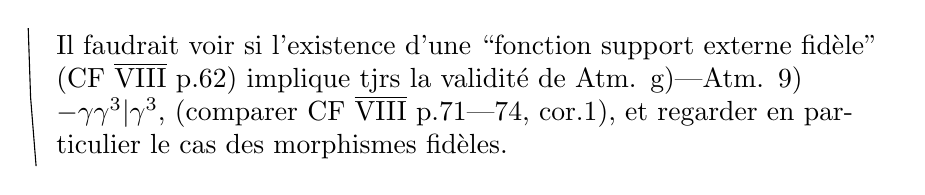
\begin{tikzpicture}
\node[anchor=north west,inner sep=0pt,text width=0.88\linewidth] (opening) at (0,0) {Il faudrait voir si l'existence d'une ``fonction support externe fidèle'' (CF \uline{$\overline{\mathrm{VIII}}$} p.62) implique tjrs la validité de \unsure{Atm. g)|Atm. 9)} $-\unsure{\gamma\gamma^3|\gamma^3}$, (comparer CF \uline{$\overline{\mathrm{VIII}}$} p.\unsure{71|74}, cor.1), et regarder en particulier le cas des \unsure{morphismes} fidèles.};
\draw ([xshift=-0.35cm,yshift=0.08cm]opening.north west) -- ([xshift=-0.32cm]opening.west);
\draw ([xshift=-0.32cm]opening.west) -- ([xshift=-0.25cm,yshift=-0.08cm]opening.south west);
\end{tikzpicture}}

Mais avant tout, il me faudrait aller de l'avant, pour me rendre compte exactement comment vont intervenir les axiomes des supports, et s'ils \deleted{sont}\inserted{s'avèrent} aussi cruciaux que je le pressens.

\figure{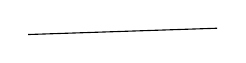
\begin{tikzpicture}\draw (0,0) -- (2.4,0.08);\end{tikzpicture}}

Critique philosophique de cette approche vers les supports, via les ``spatios'' ou ``\unsure{espacons|espaces}''. Dans la définition même des opérations essentielles $\unsure{\operatorname{co\!-\!sup}^{0}|\operatorname{co\!-\!sup}^{\circ}}$, $\unsure{\perp|\lrcorner}-\operatorname{sup}^{0}$, on est forcé de ``composer'' des strates qui ne sont pas néc. compatibles, ni même ``commensurables'' (\unsure{spectralement} disons, et encore moins combinatoirement). Or il semble \unsure{qu'on|qu'en}

\scanpage{125}
\mspage{119}
% archive sheet number: 124

fin de compte, je ne suis intéressé aux supports et opérations sur les supports, que dans le cas des supports constructibles (ou ``ens. constr.'' --- \unsure{en ajoutant} encore $\unsure{\ell|\complement}\operatorname{supp}^{\unsure{0|\circ}}\unsure{\Phi|\varphi|\phi}$\ldots), et des familles comm. de tels supports.

Il y a \deleted{\unsure{donc}} là une contradiction interne, qui reste non résolue pour le moment. D'ailleurs, même la donnée \unsure{primitive} $X\unsure{\mid\circ\mid|\mid0\mid}Y$ implique la comparaison \unsure{de|des} strates $X,Y$ qui (alors $=$ qu'elles soient ``int. disj.'') peuvent ne pas être compatibles, ni même commensurables.

Pourtant, il semble indispensable d'avoir une description 'intrinsèque' des supports \unsure{subordonnés} à une figure, comme objet d'un ens. (en l'occurrence $\Sigma_{\unsure{\mathcal A|A}}$) \uline{indépendant} de ladite figure. On va \unsure{jeter|faire}
